\documentclass[12pt, twoside]{report}
\usepackage[a4paper,left=2cm, right=2cm, top=3cm,bottom=2cm]{geometry}
\usepackage[utf8]{inputenc}

\usepackage[english]{babel}
\usepackage{amsmath}
\usepackage{graphicx}
\usepackage{textcomp}
\usepackage{parskip}
\usepackage[colorinlistoftodos]{todonotes}
\usepackage{csquotes}
\usepackage{float}
\usepackage[backend=biber,style=ieee]{biblatex}
\usepackage{hyperref}
\usepackage{graphicx}
\usepackage{epsfig}
\usepackage{caption}
\usepackage{ragged2e}
\usepackage{subcaption}
\usepackage[singlespacing]{setspace}
\usepackage{hyperref}
\usepackage[utf8]{inputenc}
\usepackage[backend=biber,style=ieee]{biblatex}
\usepackage[paper=portrait,pagesize]{typearea}
\usepackage{pdflscape}
\usepackage{hyperref}

\usepackage{biblatex}

\usepackage{diagbox} %table split headers
\usepackage{longtable} %multi-page tables

\newcommand{\tabred}{-4pt}
\newcommand*\rot{\rotatebox[x=1.32cm]{90}}

\usepackage{makecell}



%\addbibresource{friedt.bib}
\addbibresource{OCT_ref.bib}
\setlength {\marginparwidth }{2cm} 

%Chapter and name in the same line
\usepackage{titlesec}
\titleformat{\chapter}[hang] 
{\normalfont\huge\bfseries}{\chaptertitlename\ \thechapter:}{1em}{} 

\titleformat{\chapter}[display]
  {\normalfont\bfseries}{}{0pt}{\Huge}
  

\usepackage{listings}
\definecolor{mygreen}{rgb}{0,0.6,0}
\definecolor{mygray}{rgb}{0.5,0.5,0.5}
\definecolor{mymauve}{rgb}{0.58,0,0.82}
\lstset{ 
  language=Octave,
  backgroundcolor=\color{white},
  basicstyle=\footnotesize,       
  breakatwhitespace=false,         
  breaklines=true,
  captionpos=b,
  commentstyle=\color{mygreen},    
  deletekeywords={...},         
  escapeinside={\%*}{*)},        
  extendedchars=false,              
  frame=single,	                  
  keepspaces=true,                 
  keywordstyle=\color{blue},                       
  morekeywords={*,...},          
  numbers=left,                    
  numbersep=5pt,                   
  numberstyle=\tiny\color{mygray}, 
  rulecolor=\color{black},        
  showspaces=false,               
  showstringspaces=false,        
  showtabs=false,                
  stepnumber=1,                    
  stringstyle=\color{mymauve},     
  tabsize=2,	                   
  title=\lstname                   
}




\begin{document}


\lstset{language=Octave}
\begin{titlepage}

\newcommand{\HRule}{\rule{\linewidth}{0.5mm}}
\center 

\textsc{\LARGE Université Bourgogne Franche-Comté}\\[1.5cm] 
\textsc{\Large Master 2 in Smart Integrated Systems}\\[0.5cm] 

\HRule \\[0.4cm]
{ \huge \bfseries Report Innovation}\\[0.4cm] 
\HRule \\[1.5cm]


\includegraphics[scale=0.3]{logo_ubfc.png}\\[1cm]

\begin{center}
\begin{tabular}{ c   |   c } 
   
    %Opcion 2:
    ARUQUIPA Grover & \normalsize \href{mailto:grover.grover_aruquipa_aruquipa@edu.univ-fcomte.fr}{grover.grover \textunderscore aruquipa \textunderscore aruquipa@edu.univ-fcomte.fr}\\
    GASSER Florian &  \normalsize \href{mailto:florian.gasser02@edu.univ-fcomte.fr}{florian.gasser02@edu.univ-fcomte.fr}\\
    RIVERA Carlos &  \normalsize \href{mailto:carlos_manuel.rivera_aguilar@edu.univ-fcomte.fr}{carlos\textunderscore manuel.rivera\textunderscore aguilar@edu.univ-fcomte.fr}
    
\end{tabular}
\end{center}

\vfill
{\large \today}\\[1cm] 
\vfill 

\end{titlepage}
 

%\thispagestyle{empty}
%\tableofcontents
%\listoffigures
%\pagebreak


\chapter{General introduction}

This report aims to present four different applications and how they can be improved using the TRIZ method. The four applications that will be discussed include the SMark intelligent buoy, ice cube trays, Tango cane, and Gripper from a parallel robot. Each application has its own unique set of challenges and limitations, but by using the TRIZ method, we can identify potential areas for improvement and propose innovative solutions to enhance their functionality. The TRIZ method is a systematic problem-solving method that uses a combination of logic and creativity to find solutions to technical problems. By applying this method, we can find new and effective ways to improve each of these applications.

The report will be divided into four main sections, one for each application, and will include a technical section and problem and solution with the TRIZ method. In the technical section, we will describe the current design and features of each application, analyze their strengths and weaknesses and identify areas for improvement. The problem and solution section will use the TRIZ method to extract the underlying problems and identify technical contradictions. The report will then use the contradiction matrix (TRIZ) to find an innovative solution that addresses these issues.

In addition, the report will take into account the user's needs and will evaluate the solutions from a usability and accessibility perspective. Finally, the report will conclude with a summary of the key findings and recommendations for future developments. Technical terms and graphic representations will be used throughout the report to aid understanding.\\

% Involvement of each student in this report (ARUQUIPA Grover 40 percent, Gasser Florian 40 percent and RIVERA Carlos 20 percent).
Fuck off Florian XD
Fuck you too Carlos :)

\chapter{Project 1 -  Smart Mark} 
\section{Introduction}
Florian 

The aim of this project 1 is to introduce and examine the invention of the SMark intelligent buoy, and its potential to revolutionize the world of water sports. The SMark buoy is a modular, GPS controlled robotic device that can be used to set up regatta courses with precision and ease. It is lightweight, easy to assemble and can be controlled remotely using a GSM connection and an accompanying app. It can be configured with different attachments, such as an inflatable pyramid or windsock.

This report will delve into the details of the SMark buoy, including its features, capabilities and limitations. Additionally, we will use the TRIZ method to identify potential areas for improvement and propose innovative solutions to enhance the device's functionality. We will conclude with a summary of the key findings, and recommendations for future developments.

The report will be divided into two main sections: a technical section, and problem and solution with TRIZ method. The technical section will consist of two parts, the first one will describe the current invention and its features, the second one will analyze the improvement suggested using the TRIZ method. Throughout the report, we will use technical terms and graphic representations to aid the understanding of the concepts discussed.

\section{Technical section}
\subsection{Existing system}

The SMark buoy, also known as the Smart Mark, is a robotic buoy designed for setting up regatta courses, swimming competitions, and other water sports requiring a mark to signal the track. With its lightweight design, precision GPS, and remote control capabilities, the SMark buoy offers a convenient and efficient solution for course marking on the water. Additionally, its modular design allows for the use of different attachments such as a windsock, inflatable pyramid, or flashing light, making it adaptable to different types of events and competitions.

\subsubsection{Design and contruction}

The SMark buoy is designed to be lightweight and portable, with a weight of less than 15 kg, it can be easily carried by one person and put on an RIB from the water. It is made of durable and waterproof materials, and can be assembled in minutes. It is designed to withstand winds up to 20 knots and has two electric motors that keep it in place within a meter. The buoy's configuration is modular, both for energy and for the top visible part, allowing the user to choose between different attachments such as a windsock, inflatable pyramid, or flashing light.

\subsubsection{Control and navigation}

The SMark buoy is controlled remotely via GSM or Bluetooth connection, and can be set to the desired position from anywhere. It has a precision GPS that keeps it in place within a meter, and it communicates via GSM and Bluetooth, so it can be set from anywhere to the desired position. The buoy has a physical intuitive button "stay here" which helps to maintain its position.

\subsubsection{Precision and autonomy}

The buoy has a precision of within a meter, and it can last more than 12 hours with 20 knots of wind (windsock configuration) with one standard battery of 16Ah. With two standard batteries (2x 16Ah), the buoy can hold its position for 10 hours with 20 kn wind with the inflatable pyramid top. The buoy has a place for additional batteries for long autonomy.


\subsubsection{Applications and uses}

The SMark buoy is a versatile and innovative solution for setting up regatta courses on the water, and it can be used in a wide range of water sports and activities. In sailing, the buoy can be used to set up courses for races, allowing sailors to navigate and compete with precision. The buoy's precision GPS ensures that the course is marked accurately, and its remote control capabilities allow for quick and easy changes to the course as needed. The buoy's modular design also allows for the use of different attachments such as a windsock, inflatable pyramid, or flashing light, making it adaptable to different types of races and weather conditions.

In windsurfing, the buoy can be used to mark the location of obstacles, or to indicate the starting and finishing points of a race. The buoy's lightweight design and easy portability make it ideal for use in windsurfing competitions, and its precision GPS ensures that the course is marked accurately.

In swimming competitions, the buoy can be used to mark the course and ensure that swimmers stay on track. The buoy's precision GPS ensures that the course is marked accurately, and its remote control capabilities allow for quick and easy changes to the course as needed.

Additionally, the buoy can also be used for other water-based activities such as kayaking, paddleboarding, and even for rescue operations and search and rescue missions. The buoy's precision GPS and remote control capabilities make it an ideal tool for these types of activities, as it can be easily placed in the desired location and its position can be monitored and adjusted as needed.

The buoy's modular design also allows for the use of different attachments such as a windsock, inflatable pyramid, or flashing light, making it adaptable to different types of events and competitions. The buoy can be used in different weather conditions, and it is suitable for both daytime and nighttime use.

\subsection{Problem and Solution Analysis using TRIZ for Improving SMark}

In this section, we will use the TRIZ (Theory of Inventive Problem-Solving) method to identify the problems and propose solutions for improving the SMark in its design, construction, control, navigation, and application aspects.\\
First, the step of identifying and formulating a technical contradiction is applied by analyzing the SMark's current design and identifying the conflicting factors that limit its performance.

\subsubsection{Design and Construction}

\textbf{Problem 1:} Difficulty in maintaining the SMark in a fixed position during windy conditions.
This problem is the result of a technical contradiction between the need for stability and the limitation of the SMark's weight and wind resistance.

\textbf{Solution 1 :} To address this problem, we can be equipped with a more advanced GPS system and additional stabilization features such as fins or a keel. Additionally, the use of advanced control systems such as autonomous navigation can be considered to improve the SMark’s ability to maintain its position. Another solution can be to increase the weight of the SMark by adding ballast tanks that can be filled with water as needed to improve stability.

\textbf{Problem 2:} Difficulty in ensuring the durability of the SMark in harsh marine environments
This problem is the result of a technical contradiction between the need for durability and the limitation of the SMark's resistance to corrosion and wear and tear.

\textbf{Solution 2:} To address this problem, the SMark can be designed using corrosion-resistant materials such as stainless steel or aluminum, and protective coatings can be applied to the SMark's surfaces to improve its resistance to wear and tear. Additionally, the use of advanced materials such as composite materials can be considered to increase the SMark's durability.


\subsubsection{Control and Navigation}

\textbf{Problem 1:} Difficulty in controlling the SMark remotely.\\
This problem is the result of a technical contradiction between the need for remote control and the limitations of the SMark's current control system.

\textbf{Solution 1:} To address this problem, the SMark can be equipped with a web interface and wireless control system that allows for remote control of its movement and signaling systems. Then, the use of advanced technologies such as artificial intelligence and machine learning can be considered to optimize the control of the SMark. Another solution can be to add a joystick or other hand-held control device that can be used to remotely control the SMark’s movement and signaling systems.

\textbf{Problem 2:} Difficulty in providing accurate navigation information in low visibility conditions.\\
This problem is the result of a technical contradiction between the need for accurate navigation information and the limitations of the SMark's current navigation system in low visibility conditions.

\textbf{Solution 2:} To address this problem, the SMark's navigation system can be upgraded with advanced features such as radar, sonar, or Lidar to provide real-time navigation information. A heads-up display or other augmented reality system can be added to the SMark to provide real-time navigation information to competitors and organizers. Additionally, the use of advanced navigation technologies such as GPS and inertial navigation systems can be considered to improve the accuracy of the SMark.

\subsubsection{Application and Utilization}

\textbf{Problem 1:} Difficulty in adapting the SMark to different water sports.\\
This problem is the result of a technical contradiction between the need for adaptability and the limitations of the SMark's current design.

\textbf{Solution 1:} To address this problem, the SMark can be designed with a modular concept that allows for easy customization and adaptation to different water sports and weather conditions. Additionally, the use of advanced materials and technologies such as shape memory alloys or smart materials can be considered to allow the SMark to adapt to different water sports and weather conditions.

\textbf{Problem 2:} Difficulty in providing adequate safety features for competitors and organizers.\\
This problem is the result of a technical contradiction between the need for safety and the limitations of the SMark's current safety features.

\textbf{Solution 2:} To address this problem, the SMark can be equipped with additional safety features such as emergency stop buttons and automatic weather alerts. Then, the use of advanced technologies such as sensors and monitoring systems can be considered to provide real-time safety information to competitors and organizers. Another solution can be to add a rescue beacon or other emergency signaling device to the SMark to provide real-time safety information in case of emergency.\\

In summary, by identifying and formulating the technical contradiction through the TRIZ method, we can more effectively analyze and solve the problems related to the SMark invention. By identifying the conflicting factors and proposing solutions to overcome them, we can improve the overall performance and functionality of the SMark for use in water sports and ensure the safety of competitors and organizers.



\section{TRIZ Table}

According to the previous contradictions, we can find the important contradictions in the \textbf{TRIZ} table, which will help us find the correct parameters in order to apply the improvement for this device.
\begin{table}
[H]\centering\setlength\tabcolsep{5.5pt}\renewcommand\arraystretch{1.25}
  \noindent\makebox[\textwidth]{%
    \begin{tabular}{|l|*{3}{c|}}
      \hline
      \diagbox[width=\dimexpr \textwidth/8+3\tabcolsep\relax, height=2cm]{ Improvement }{Weakening}
                   & Complexity of the device & Shape & Repair ability \\
      \hline
      Adaptability, Fiability, stability & 13,14,27, 37 & 15, 37, 1 & 1, 19\\
        \hline
        
    \end{tabular}
    \label{Tab:First_contradiction2}

  }%
  \caption{First contradiction analysis}

\end{table}

\begin{table}[H]\centering\setlength\tabcolsep{5.5pt}\renewcommand\arraystretch{1.25}
  \noindent\makebox[\textwidth]{%
    \begin{tabular}{|l|*{1}{c|}}
      \hline
      \diagbox[width=\dimexpr \textwidth/8+3\tabcolsep\relax, height=2cm]{ Improvement }{Weakening}
                   & Reliability \\
      \hline
      Shape & 6,1\\
      \hline
       Performance & 14, 18, 21\\
      \hline 
       Ility & 36,37,38,39\\
      \hline
       Manufacture  & 43,46, 45\\
       \hline
       Measurement & 47,48\\
       \hline
    \end{tabular}
    \label{Tab:Second_contradiction2}
  }%
  \caption{Observed problems}
\end{table}

In order to apply the principles, we can define the  principles which can be applied to this case as:\\

\begin{itemize}
\item \textbf{Adaptability and Reliability :}
\subitem Multi-Functionality
\subitem Self-Service
\subitem Self-Recovery
\item \textbf{Stability :}
\subitem Counterweight
\subitem Inertial System
\subitem Oscillation Damping
\item \textbf{Shape :}
\subitem Continuously Variable Shape
\subitem Combining Solids and Liquids
\subitem Elasticity
\item \textbf{Performance :}
\subitem Segmentation
\subitem Homogeneity
\subitem Homogenization
\item \textbf{Manufacture :}
\subitem Micro-Miniaturization
\subitem Structural Changes
\subitem Local Quality
\item \textbf{Measurement :}
\subitem Substitution
\subitem Anti-Selection
\subitem Inverse Effect
\end{itemize}


\section{Solution Proposed}

Using the previous \textit{TRIZ} table, we can define the following possible solutions in order to improve this device, based on incentive principles detected previously.

\begin{itemize}
\item Apply advanced GPS system with additional stabilization features such as fins or a keel to improve the SMark’s ability to maintain its position. This will help to overcome the difficulties in maintaining the SMark in a fixed position during windy conditions.
\item Use advanced control systems such as autonomous navigation to further improve the SMark’s ability to maintain its position. This will also help to overcome the difficulties in controlling the SMark remotely.
\item Use advanced materials and technologies such as shape memory alloys or smart materials to allow the SMark to adapt to different water sports and weather conditions. This will help to overcome the difficulties in adapting the SMark to different water sports.
\item Add a rescue beacon or other emergency signaling device to the SMark to provide real-time safety information in case of an emergency. This will help to overcome the difficulties in providing adequate safety features for competitors and organizers.
\item Use a modular concept that allows for easy customization and adaptation to different water sports and weather conditions. This will help to overcome the difficulties in adapting the SMark to different water sports and weather conditions.
\item Use advanced technologies such as sensors and monitoring systems to provide real-time safety information to competitors and organizers. This will help to overcome the difficulties in providing adequate safety features for competitors and organizers.
\item Use a remote-controlled deployment system to allow for easy installation without the need for manual labor. This will help to overcome the difficulties in transporting and storing the SMark.
\item Use an inflatable design to make the SMark more portable and easy to store when not in use. This will help to overcome the difficulties in transporting and storing the SMark.
\item Use advanced navigation systems such as radar, sonar, or Lidar to provide real-time navigation information. This will help to overcome the difficulties in providing adequate navigation information for competitors and organizers.
\end{itemize}

\begin{figure}[H]
    \centering
    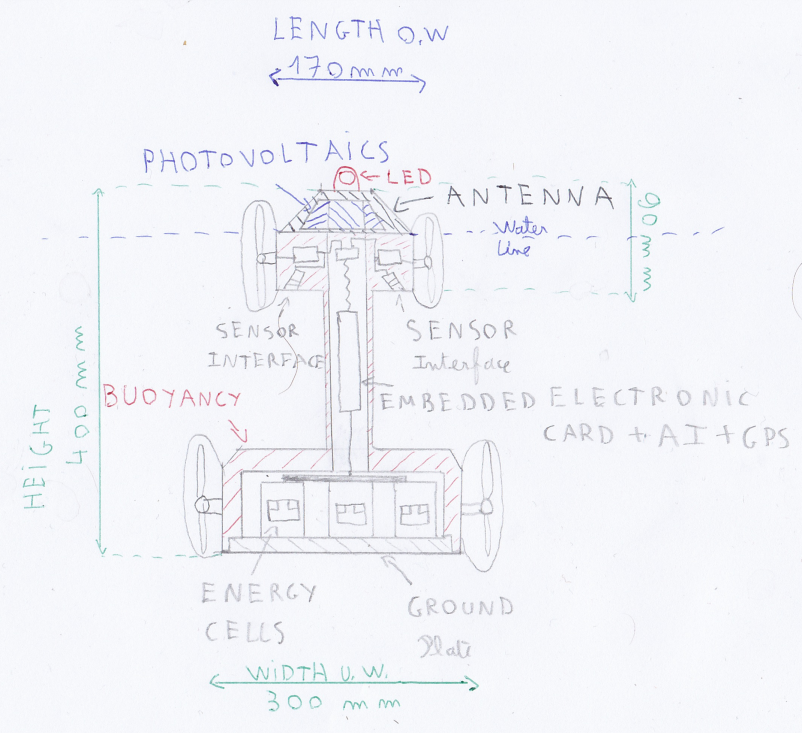
\includegraphics[width=150mm,scale=1]{images/sketch.PNG}
    \caption{Sketch about smart buoy}
    \label{fig:smart}
\end{figure}

The solution proposed in Fig. \ref{fig:smart}, shows the complete assembly of the system, which is proposed as a solution to the problems found. The TRIZ method has allowed to find an optimal solution for the design in this type of system.


\section{Conclusion}

In conclusion, the SMark robotic buoy invention presents several problems in its design, construction, control, navigation and application aspects. However, by using the TRIZ method, we were able to identify these problems and propose solutions for improvement. The most important contradictions in this invention are related to the complexity of the device, the shape, and the repairability. To overcome these issues, we proposed solutions such as upgrading the GPS system, adding stabilization features, designing the SMark to be more compact and lightweight, and incorporating advanced technologies such as autonomous navigation and artificial intelligence.\\

we suggested the use of advanced materials and technologies such as shape memory alloys and smart materials to improve the adaptability of the SMark to different water sports and weather conditions. Overall, by implementing these solutions, we can enhance the performance, reliability, and safety of the SMark, making it more suitable for use in water sports competitions.

\newpage
\chapter{Project 2- \LARGE A new ice cube tray for the adhesion of liquids}
Grover
\section{Introduction}
The Ice cube trays are a common feature in many refrigerators, but they can cause problems for some users. Some of these issues include:
\begin{itemize}
    \item Ice cubes sticking to the tray and making it difficult to remove them.
    \item Not enough space in the fridge for multiple ice cube trays, or not enough space between the shelves to fit them all at once.
    \item Trays that are too small, resulting in thin ice cubes that melt quickly or don't have much flavor when used in drinks or food dishes such as cocktails and smoothies.
    \item Ice cubes with an unpleasant taste due to impurities from the water supply being frozen into the cubes themselves during the freezing process.
\end{itemize}
These common issues can be resolved by selecting the right type of ice cube tray for your needs. For example, larger trays may help with space constraints and silicone trays are easier to remove cubes from than plastic ones. Selecting a tray that is made from food-safe materials will also ensure that any impurities in the water supply don't end up in the cubes themselves. Finally, making sure to store the trays away from cold air sources such as vents or near walls can reduce frost buildup on them.

The main objective in this section is to improve the ice cube try, using the TRIZ method, in order to find the best solution for this common component in a refrigerator. Firstly is identified the previous designs, after is extracted the problem in these systems, in order to find the technical contradictions, and finally using the contradiction matrix (\textit{TRIZ}) we can find an innovation solution.

\section{Technical section}
\subsection{Existing Systems}

Previously there is presented a group of systems from different companies, where we can find systems which helps to solve the possible issues in the system, we summarize the existed systems as is observed below:\\
\begin{itemize}
    \item \textbf{REFRIGERATOR, REFRIGERATOR MANAGEMENT SYSTEM AND METHOD FOR CONTROLLING THE WATER SUPPLY TO AN ICE CUBE TRAY IN A REFRIGERATOR}

This is a 2020 patented ice maker having a base and a separate side extending from the base to define an opening opposite the base, and having a divider extending from the base and/or at the bottom. separate side to divide the container into at least two compartments for making ice. The container is a container that can be closed by means of zipper elements that extend from the inner sides of the opening.\\
The opening can be deformed between open and closed configurations, and the first and second zipper elements can be disengaged when the opening is open and engaged when the opening is closed, the container can be molded from platinum silicone as a unitary assembly without parts attached according to the manufacturer. The molding process can be liquid injection molding, compression molding or transfer molding, Fig. \ref{fig:model1} shows this container in its CAD drawing.

\begin{figure}[H]
    \centering
    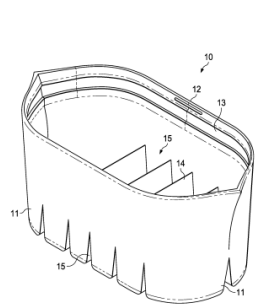
\includegraphics[width=50mm,scale=0.8]{images/Project2/innovation1.png}
    \caption{Model 1}
    \label{fig:model1}
\end{figure}

The patent link can be seen in \footnote{\href{https://data.inpi.fr/brevets/WO2020185345}{Ice cube tray 1}}


\item \textbf{SOFT CONTAINER WITH ICE CUBE TRAY}

This patent shows a component comprising: a door opening/closing history storage unit for storing refrigerating room door opening/closing information and opening/closing time detected by a detection unit door open/close as a door open/close history; a replenishment judgment information storage unit for storing, as replenishment judgment information, the opening/closing history of the refrigeration room door in which replenishment of water of a tank is judged to have occurred ice bin water storage.\\
A judging unit for judging whether replenishment of water of the ice bin water storage tank has occurred, the judging being performed based on the door opening/closing history stored in the opening/closing history storage unit gate and reset judgment information stored in the reset judgment information storage unit.\\
Additionally, a judging unit for judging whether the ice tray water storage tank is empty based on the judging result of whether water replenishment has occurred as estimated by the judging unit, the refrigerator being such that a water supply control unit does not control the supply of water to a water supply pump when the evaluation unit has determined that the ice cube tray of the water storage tank is empty. Therefore, it is possible to suppress performing unnecessary operations for supplying water to an ice cube tray. Fig \ref{fig:model2} shows this model.
\begin{figure}[H]
    \centering
    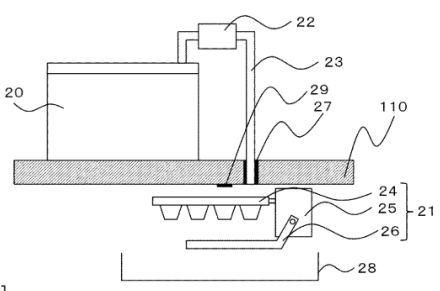
\includegraphics[width=50mm,scale=0.5]{images/Project2/innovation2.png}
    \caption{Model 2}
    \label{fig:model2}
\end{figure}
    
The patent link can be seen in \footnote{\href{https://data.inpi.fr/brevets/WO2020129242}{Ice cube tray 2}}

\item \textbf{ICE TRAY-22/04/2021}

This component presents an ice tray comprising a body; a plurality of cavities arranged in the body and having space to receive water and convert it into ice; an opening formed in the body for supplying water to the cavities or for extracting ice formed therein; and a lid to close the opening.\\
The plurality of cavities includes a plurality of first cavities that are arranged along the vertical direction and are in communication with each other, and the opening includes a first opening that is in communication with the first cavities. The Fig. \ref{fig:model3} shows this model.

\begin{figure}[H]
    \centering
    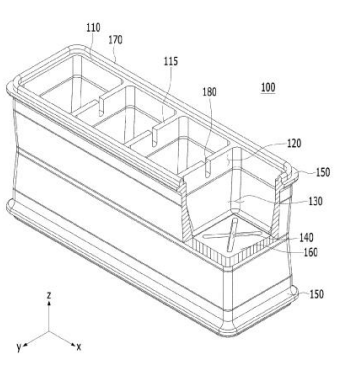
\includegraphics[width=50mm,scale=0.5]{images/Project2/innovation3.png}
    \caption{Model 3}
    \label{fig:model3}
\end{figure}
The patent link can be seen in \footnote{\href{https://data.inpi.fr/brevets/WO2022225130}{Ice cube tray 3}}

    
\end{itemize}


\section{Problem and solutions}

The main problem that we will seek to improve will be the difficulty of extracting or separate the cubes, additionally there is not contemplate other problems such as different liquids.\\
\begin{figure}[H]
    \centering
    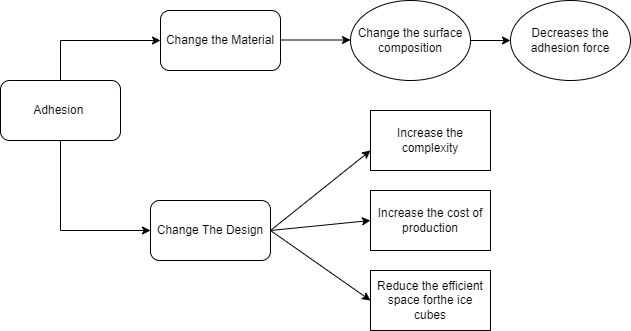
\includegraphics[width=100mm,scale=0.8]{images/EXERCISE_2/iccubes.drawio.png}
    \caption{Problem diagram}
    \label{fig:problem_Diagram}
\end{figure}

In order to explore the possible solutions for the design, the possible point of views problems are observed as following:\\
\begin{itemize}
    \item Find a solution to minimize the adhesion forces with the surfaces
    \item Find a way to obtain an efficient design
    \item Find a way to increase the volume of the product.
    \item Find a design with material reduction 
\end{itemize}
 \textit{Additionally it is necessary to solve the following contradictions:}
\begin{itemize}
    \item If we  change the material we will lose the sliding shape, If we change the material we will change the weight of the material.
    \item If we change the design we will lose the manufacturing precise, if we change the design we will increase the complexity
    \item If we increase the volume we will increase the stability
    \item If we change the Design we will decrease the reliability
\end{itemize}
 
%%%%%%%%%%%%%%%%%%%%%%%%%%%%%%%%%%%
%%%%%%%%%%%%%%%%%%%%%%%%%%%%%%%%%%%
\section{Triz Table}
According to the previous contradiction, we can find the most important contradictions in the \textbf{TRIZ} table, which will help us find the correct principle of invention in order to apply the improvement for this device.

\begin{table}
[H]\centering\setlength\tabcolsep{5.5pt}\renewcommand\arraystretch{1.25}
  \noindent\makebox[\textwidth]{%
    \begin{tabular}{|l|*{3}{c|}}
      \hline
      \diagbox[width=\dimexpr \textwidth/8+3\tabcolsep\relax, height=2cm]{ Improvement }{Weakening}
                   & Complexity of the device & Shape & Repair ability \\
      \hline
      Adaptability or Versatility& 15, 29, 37,28 & 15, 37, 1 , 8 & 1, 16, 7, 4\\
        \hline
        
    \end{tabular}
    \label{Tab:First_contradiction2}

  }%
  \caption{First contradiction analysis}

\end{table}

\begin{table}[H]\centering\setlength\tabcolsep{5.5pt}\renewcommand\arraystretch{1.25}
  \noindent\makebox[\textwidth]{%
    \begin{tabular}{|l|*{1}{c|}}
      \hline
      \diagbox[width=\dimexpr \textwidth/8+3\tabcolsep\relax, height=2cm]{ Improvement }{Weakening}
                   & Reliability \\
      \hline
      Shape & 10, 40, 16\\
      \hline
      Manufacturing Precision & 11, 32, 1\\
      \hline 
      Ease of Manufacture & --\\
        \hline
    \end{tabular}
    \label{Tab:Second_contradiction2}
  }%
  \caption{Observed problems}
\end{table}
Second, to apply these principles, we can define the  principles which can be applied, for this case as shown below:\\
\begin{itemize}
    \item \textbf{Complexity of the Device:}
    \subitem Dynamics
    \subitem Pneumatic
    \subitem Thermal Expansion
    \item \textbf{Shape}
    \subitem Flexible Films
    \subitem Composite Material
    \item \textbf{Repair Ability}
    \subitem Division
    \subitem Asymmetric
    \subitem Embedded Structure
\end{itemize}
Using the previously associated incentive principles, we can point out that to improve the versatility of the ice cube system, the complexity of the product will increase by affecting the parameters of \textit{(Dynamic, Pneumatic and thermal expansion)}, in the same way the Shape affects will take into account the principles of incentive for flexibility films and composite materials. Secondly, the principle of incentive Repair ability directly affects the division, asymmetry and the embedded structure.


\section{Solution Proposed}
Using the previous \textit{TRIZ} table, is defined the following possible solutions in order to improve this device, based on incentive principles detected previously.
\begin{itemize}
    \item Use a non-stick material, such as silicone or Teflon, to make the ice cube tray. This will reduce adhesion and make it easier for cubes to be removed from the tray, in this way it can be added in Fig. \ref{fig:sol21x}.
    \item Apply a thin layer of wrinkled surface on the inside of the tray before pouring in water to create the ice cubes. This will also help prevent sticking and allow for easy removal when frozen solid.
    \item Place an upside down plate over top of the filled ice cube trays and press lightly with your hands before placing them into the freezer - this helps ensure that all cubes freeze evenly without any sticking together due to uneven surfaces in certain areas of your tray, so this design is observed in the Fig. \ref{fig:Assemb2}.\\
    Where we can observe the complete assembly, although in the first Figure, holes are observed, these are slightly filled by the other component, in such a way that the extraction is quick and simple, this solution can be considered new by looking at the state of the art it is not possible to find a similar design. 
\end{itemize}

%Superficie corugada
\begin{figure}[H]
    \centering
    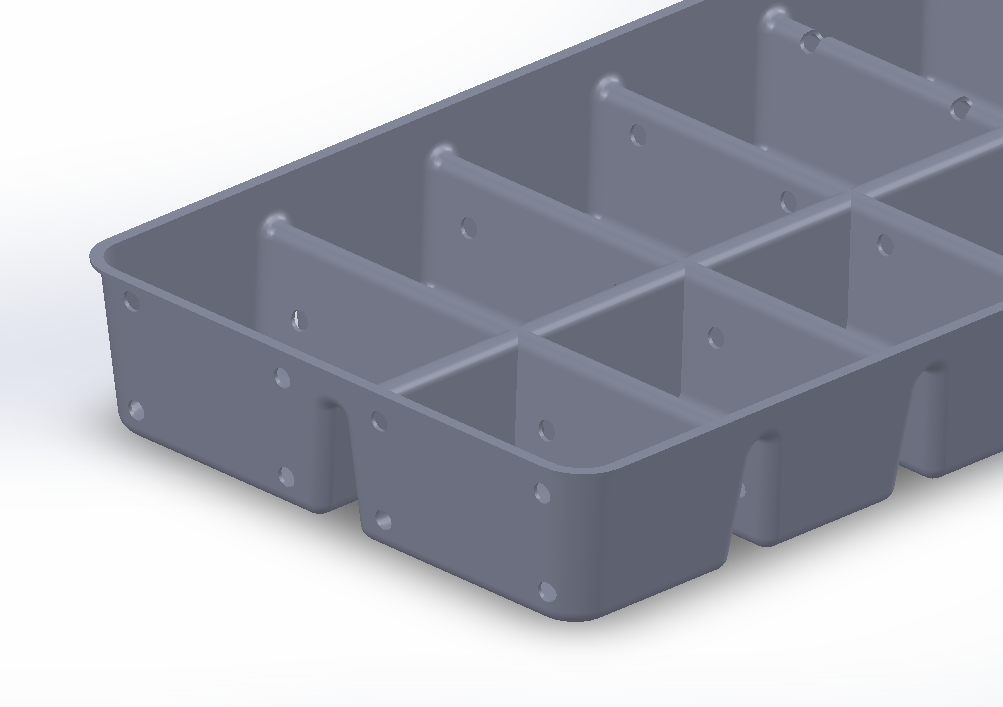
\includegraphics[width=100mm,scale=0.8]{images/Project2/innov3d1.png}
    \caption{proposed adhesion solution designed in CAD}
    \label{fig:sol21x}
\end{figure}
\begin{figure}[H]
    \centering
    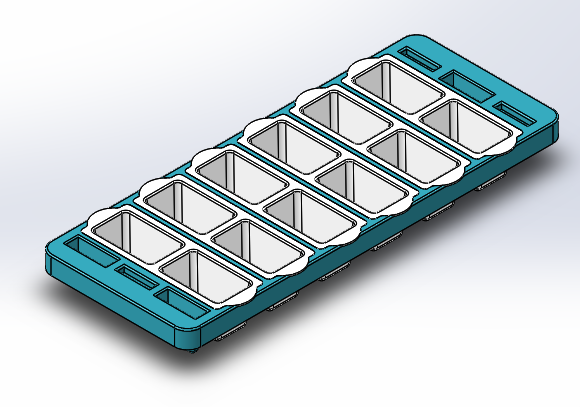
\includegraphics[width=100mm,scale=0.8]{images/Project2/cad2.png}
    \caption{Assembly Proposed adhesion solution designed in CAD}
    \label{fig:Assemb2}
\end{figure}
%%%%%%%%%
The solution proposed in Fig. \ref{fig:Assemb2}, shows the complete assembly of the system, which is proposed as a solution for the adhesion problem, from the TRIZ method it was possible to face and find a possible optimal solution for adhesion in this type of system, The designs were made using \textit{Solidworks} in such a way as to capture the basic idea.
\section{Conclusion}

This new system of ice cubes tray, that consists of a main assembly of two parts, specifically covers the problem of adhesion. The main innovation based on the parameters of corrugated surface, holes against adhesion and geometric optimization, helped to generate a good product that can potentially solve the proposed problem, based on a cost analysis that should be done based on this idea.
%%%%%%%%%%%%
% ??


\chapter{Project 3 - \LARGE Self-standing "Tango Cane".}
\section{Introduction}
The Tango cane is a popular assistive device for individuals with mobility impairments, notably seniors, providing support and stability while walking, with the added feature of being able to stand straight when let go, even withstanding external movement that may tip over a regular cane. However, as technology and the needs of users continue to evolve, there is a growing need to improve and add new features to the existing self-standing Tango cane. By using TRIZ techniques, we have envisioned a more effective and user-friendly device that better meets the needs of those who rely on it and implement innovative features based on current technologies. Some potential areas for improvement could include:

\begin{enumerate}
    \item Safety and Emergency Assistance:
    \begin{itemize}
        % \item GPS and emergency alert.
        % \item Obstacle detection.
        \item Fall detection. %%%%%%%% maybe
        % \item Vibration or sound warning of imminent fall.
    \end{itemize}

    \item Mobility and Balance Assistance:
    \begin{itemize}
        % \item Balance assistance. 
        \item Stair-climbing capability. %%%%%%%% maybe
        % \item Electric motor-assisted walking.
    \end{itemize}

    \item Convenience and Accessibility:
    \begin{itemize}
        \item Built-in light.
        % \item Mobile phone integration.
        % \item Voice commands.
        \item Foldable and lightweight design. %%%%%%%% maybe
        % \item Automatic seat.
    \end{itemize}

    \item Health Monitoring:
    \begin{itemize}
        % \item Obstacle detection.
        \item Weight-bearing sensor. %%%%%%%% maybe
        % \item Balance assistance.
        \item Electric motor-assisted walking.
    \end{itemize}
\end{enumerate}

By addressing these issues, we can create a Tango cane that is even more responsive to the needs of its users, helping them to maintain their independence and quality of life.

\section{Existing system}

The current know version of the Tango cane (figure \ref{fig:tango_org}) is designed to provide support and stability to seniors or people with mobility issues while they are standing or walking. The cane has a shape that allows it to stand upright on its own, without the need for a separate stand or holder. This feature allows the user to rest the cane on its own when not in use and have both hands free for other tasks. The cane is usually made of lightweight materials, such as aluminum or carbon fiber, to make it easy for seniors to handle and maneuver. The self-standing feature is achieved thanks to a weighted bottom with a particular shape. Additionally, the cane can come with features such as a comfortable handle, adjustable height, and a non-slip tip to ensure safety and stability.

While the self-standing cane's material and mechanical design is important, we sought to explore other areas of improvement that could be achieved through the integration of embedded systems, thereby adding more advanced features.

\begin{figure}[!h]
    \centering
    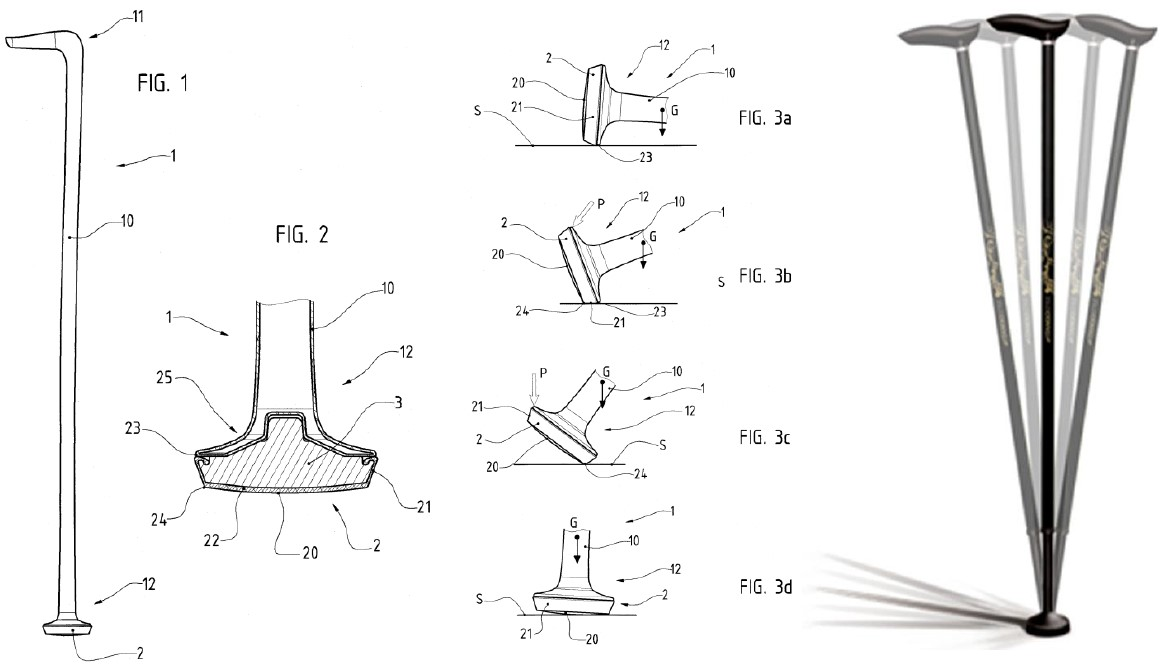
\includegraphics[width=\textwidth]{images/Project 3/tango_original.jpg}
    \caption{Diagram of Self-standing ”Tango Cane”.}
    \label{fig:tango_org}
\end{figure}

\section{Problem and solution analysis}

\begin{enumerate}
    \item Safety and Emergency Assistance:
    \begin{itemize}
        \item \textbf{Fall detection:} Falls can be particularly dangerous for seniors, as they can lead to serious injuries and even death. A cane with fall detection technology can automatically notify a designated emergency contact if the senior falls and is unable to get up. Such notification can include, thanks to a GPS module, the exact location of the incident. As a preventive measure, the cane can be equipped with a sensor capable to detect an imminent fall and, thus, generate a sound and vibration warning to the user.
    \end{itemize}

    \item Mobility and Balance Assistance:
    \begin{itemize}
        \item \textbf{Stair-climbing capability:} Navigating stairs can be challenging for seniors due to balance, strength, and mobility issues. This can lead to falls and injuries, which can be serious and even fatal. The proposed feature, can help seniors navigate stairs more easily and safely, reducing the risk of falls.
    \end{itemize}

    \item Convenience and Accessibility:
    \begin{itemize}
        \item \textbf{Built-in light:} Low-light environments can be challenging for seniors due to decreased vision and sensitivity to light, which can make it difficult to see obstacles and hazards. This can lead to falls and injuries, and can limit seniors' ability to move around safely, especially during evening hours. Having a built-in light can help seniors navigate in dark environments more easily and safely.
        \item \textbf{Foldable and lightweight design:} This feature addresses the difficulty and inconvenience associated with storing and transporting a traditional cane for seniors or people with mobility issues. Traditional canes can be bulky and heavy, making them difficult to store and carry around. This can can be especially challenging when traveling or going out in public. The feature makes it more convenient for seniors to take their cane with them wherever they go, and also makes it easier to store when not in use.
    \end{itemize}

    \item Health Monitoring:
    \begin{itemize}
        \item \textbf{Weight-bearing sensor:} The risk of falls, as previously mentioned, can be a serious issue as it can increase the risk of injuries, and can limit seniors' ability to move around and maintain their independence. A Weight-bearing sensor could detect when a senior is experiencing weakness or instability in their legs, and provide a notification to them and a designated emergency contact, allowing for early detection and management of this issue.
        
        \item \textbf{Oximeter and heart rate monitor sensors:} Seniors are more vulnerable to health-related problems and it can be hard for them to detect early signs of health issues. This feature would allow them to continuously monitor their oxygen saturation levels and heart rate, providing them with valuable information about their health early on and seek medical attention if necessary.
    \end{itemize}
\end{enumerate}

\section{TRIZ application}
\textbf{The cane should be lightweight and easy to carry, but also sturdy and durable enough to support a senior's weight and provide balance assistance.}

This is a contradiction between "lightweight" and "sturdy and durable", to resolve it the following principles can be applied:

Principle 1: Segmentation: Divide the cane into different segments that can be individually adjusted for weight and sturdiness.

Principle 8: Counterweight: Use a counterweight to balance the cane and make it easier to carry, while still maintaining its sturdiness and durability.

\textbf{The cane should have fall detection and emergency assistance features, but also be unobtrusive and not impede a senior's movement or independence.}

Principle 7: Nested doll: We could use a nested design in which the cane's fall detection and emergency assistance features are hidden inside the cane and only activated when needed.

\textbf{The cane should have a built-in light for low-light environments, but also not add excessive weight or bulk to the cane.}

Principle 29: Pneumatics and hydraulics: We may think in using a built-in light that is powered by air pressure, having a system that takes advantage of the user’s weight when walking, eliminating the need for batteries and reducing the weight and bulk of the cane.

\textbf{The cane should have the ability to navigate stairs, but also be easy to use and not add complexity to the cane.}

Principle 16: Partial or excess action: We could create a cane that can adjust the level of assistance it provides for different surfaces, including stairs, making it easy to use and not adding complexity. That is, having a retractable mechanism that adds support for the stairs but can be folded back into the cane when is not needed.

\textbf{The cane should be foldable and easy to store, but also be sturdy enough to support a senior's weight and provide balance assistance.}

Principle 3: Local Quality: Applying a folding mechanism that allows for easy storage while still maintaining the structural integrity and stability of the cane.

Principle 30: Flexible membranes and thin films: Utilizing flexible and durable materials that allow for easy folding while still maintaining the cane's strength and stability while being used.

\textbf{The cane should have fall detection and emergency assistance features, but also be affordable and accessible for all seniors.}

Principle 13: Inversion: We may invert the problem and instead of making the cane more affordable, focus on making it easier for seniors to access financial assistance to purchase the cane.

Principle 6: Multifunctionality: Invent a cane that has multiple functions, such as fall detection and emergency assistance features, as well as other features as previously described that can justify its higher cost, making it more accessible and affordable for seniors all things considered.


\section{Solution proposed}

Figure \ref{fig:cane2} displays a stair-climbing capability added to a cane, using a design in which the cane is divided in two parts, using an internal connector, is an innovative solution that allows seniors to navigate stairs more easily and safely, reducing the risk of falls. The basic concept design of this cane is that it is divided into two parts. The first part is the upper section, which is designed to be placed on top of the step of the stairs. The second part is the lower section, which stays fixed on the ground. The internal connector allows the two parts to be extended and locked into place, creating a stable and secure platform for the senior to step on as they navigate the stairs.

\begin{figure}[!h]
    \centering
    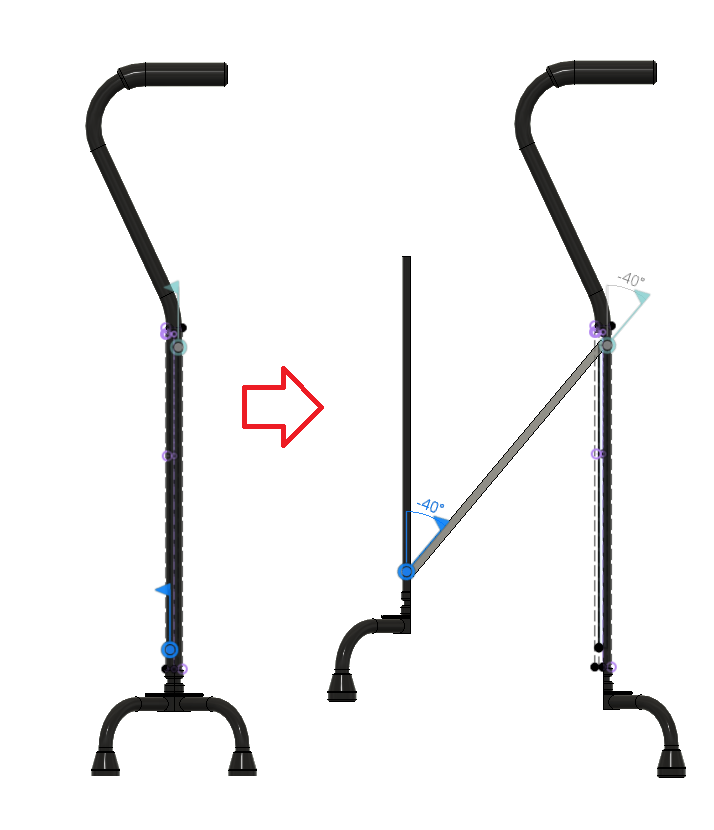
\includegraphics[width=0.75\textwidth]{images/Project 3/stairs.png}
    \caption{Basic design for the Stair-climbing capability.}
    \label{fig:cane2}
\end{figure}

This design has several advantages, such as:

Increased stability and safety: The cane is extended and locked into place, creating a stable and secure platform for the senior to step on as they navigate the stairs.
Improved balance assistance: The cane provides added support and stability when ascending and descending stairs, reducing the risk of falls.
Greater independence: This design allows seniors to navigate stairs more easily and safely, giving them greater independence and freedom of movement.
Convenience: It can be easily stored and transported, making it convenient for seniors to take it with them wherever they go.
Ease of use: The cane is easy to use, even for seniors with limited mobility or dexterity, making it accessible to a wider range of users.

The other features added to the cane such as Fall detection with GPS alert capabilities, Weight-bearing sensor and Oximeter and heart rate monitor sensors, are not displayed using Computer-Aided Design (CAD) because they consist of internal components that are not visible from the outside. These features are added to the cane as internal components and are not visible on the exterior of the cane.

The fall detection feature is a sensor system that is integrated into the cane to automatically detect when a senior has fallen and is unable to get up. This sensor system can be triggered by a variety of factors such as sudden changes in the cane's position, impact or loss of contact with the ground. When a fall is detected, the cane can automatically send an alert to a designated emergency contact, including the senior's GPS location, allowing for quick response and assistance.

The weight-bearing sensor is another internal component that is integrated into the cane. This sensor can detect when a senior is experiencing weakness or instability in their legs, and provide a notification to them and a designated emergency contact, allowing for early detection and management of this issue.

The Oximeter and heart rate monitor sensors are also internal components that are integrated into the cane. These sensors allow the senior to continuously monitor their oxygen saturation levels and heart rate, providing them with valuable information about their health early on and seek medical attention if necessary.

These features are not visible from the outside and are not included in the CAD representation of the cane, but they play an important role in the functionality and safety of the cane and its ability to assist seniors in their daily lives.

\section{Conclusion}
In conclusion, the Tango cane is a widely used assistive device for individuals with mobility impairments, particularly seniors. The cane's unique design allows it to stand upright on its own and provides support and stability while walking. However, as technology and the needs of users continue to evolve, there is a growing need to improve and add new features to the existing Tango cane. Using TRIZ techniques, new features were proposed to improve safety, mobility, convenience, and health monitoring. These features include fall detection with GPS alert capabilities, stair-climbing capability, built-in light, foldable and lightweight design, weight-bearing sensor, and electric motor-assisted walking. By addressing these issues, the Tango cane can be made even more responsive to the needs of its users, helping them to maintain their independence and quality of life.

\chapter{Project 4- \LARGE Robotic gripper improvement for safe handling}

\section{Existing Systems}

This project will try to improve the gripper using parallel mechanisms in such a way as to obtain a safe grip when handling large weight and low dimension objects.

\begin{figure}[H]
     \centering
     \begin{subfigure}[b]{0.3\textwidth}
         \centering
         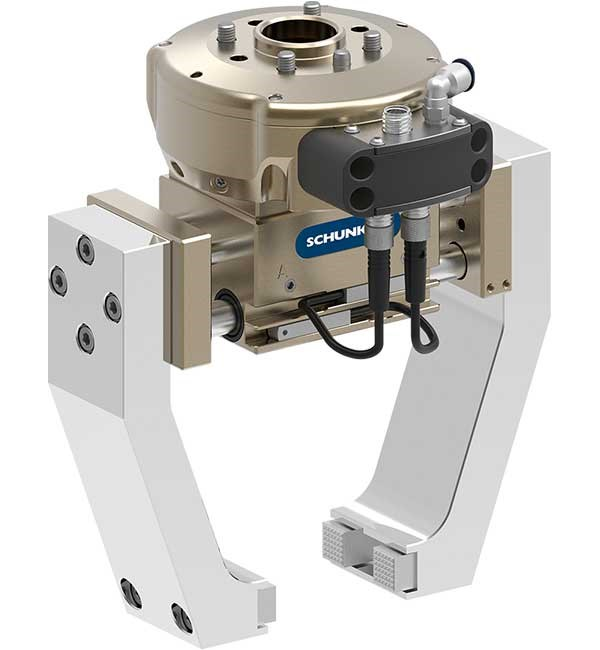
\includegraphics[width=\textwidth]{images/Project4/gripper1.jpg}
         \caption{Conventional Gripper}
         \label{fig:conv}
     \end{subfigure}
     \hfill
     \begin{subfigure}[b]{0.3\textwidth}
         \centering
         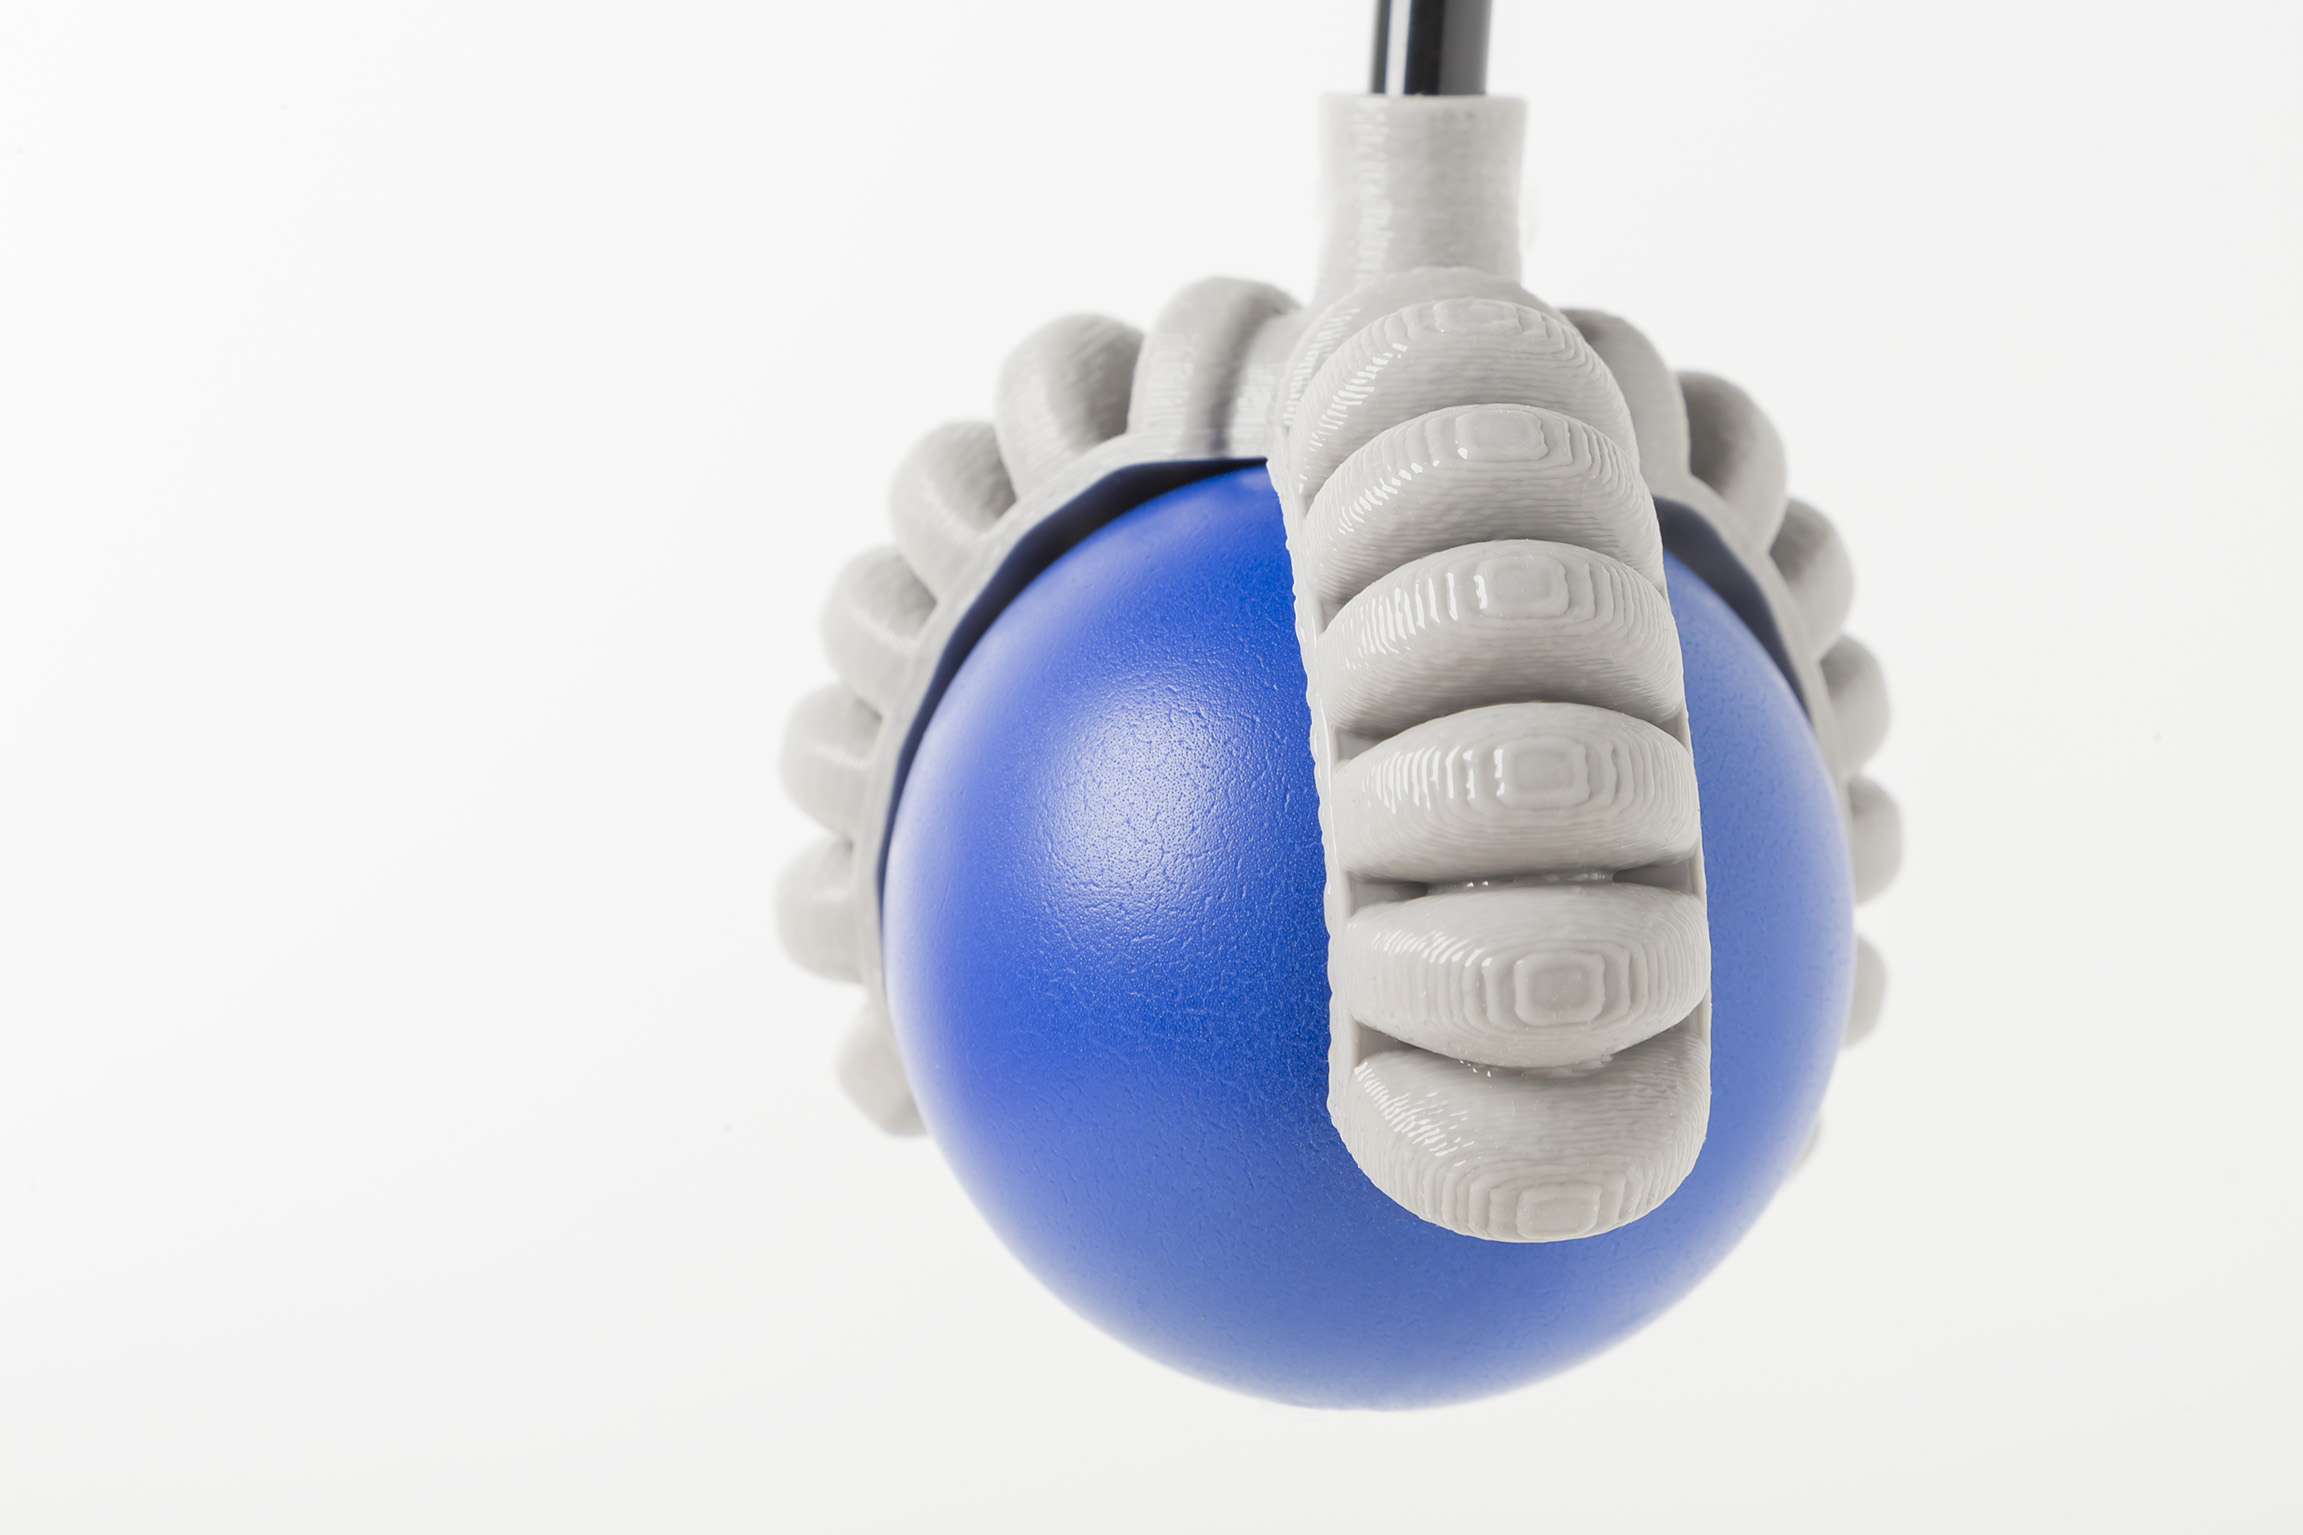
\includegraphics[width=\textwidth]{images/Project4/gripper2.jpg}
         \caption{Soft robotic Gripper}
         \label{fig:Soft_hand}
     \end{subfigure}
     \hfill
     \begin{subfigure}[b]{0.3\textwidth}
         \centering
         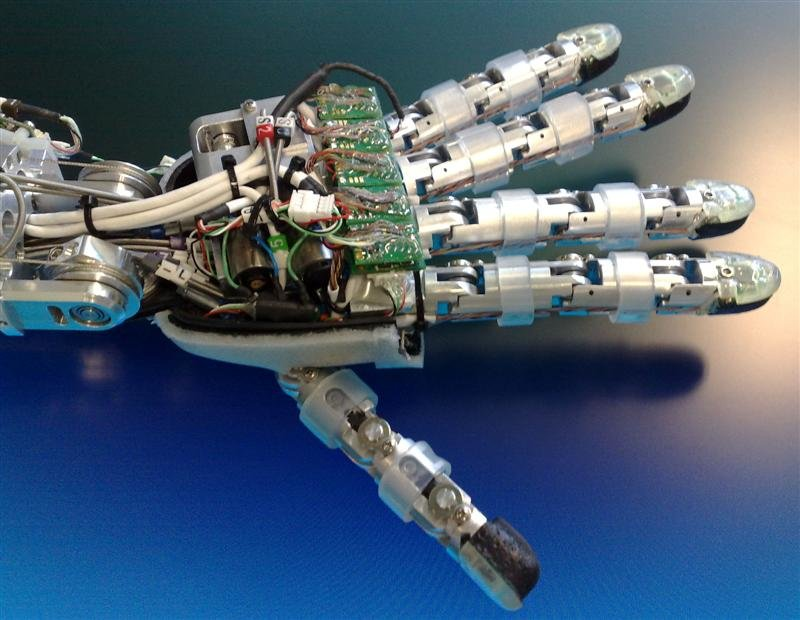
\includegraphics[width=\textwidth]{images/Project4/gripper3.png}
         \caption{Humanoid Gripper}
         \label{fig:Robotic_hand}
     \end{subfigure}
        \caption{Three simple graphs}
        \label{fig:three_Common}
\end{figure}

\subsection{Conventional Grippers}
The advantages of the conventional grippers in robotics are that they are very simple and cheap to build, and they are very versatile. They can be used to pick up a wide variety of objects of different shapes and sizes as example the Fig. \ref{fig:conv}.

The disadvantages of the conventional grippers in robotics are that they are not very strong, and they can be difficult to use to grip small objects.\\

Some of the best examples of the conventional grippers in robotics are the robotic arms used in factories. These arms are typically equipped with a number of different grippers, such as vacuum grippers and pneumatic grippers, that allow them to grip and manipulate a wide variety of objects.
\subsection{Soft Robotic Grippers}

The advantages of soft grippers in robotics are that they are able to conform to the shape of an object, which makes them ideal for gripping delicate objects. They are also lightweight and can be easily manipulated. The disadvantages of soft grippers in robotics are that they are not as strong as traditional metal grippers and they can be damaged if they come into contact with sharp objects. \ref{fig:Soft_hand}\\

Some of the best examples of soft grippers in robotics include the $Robotiq 2F Soft$ Gripper, the $Festo$ Soft Gripper, and the $chunk$ Pneumatic Gripper. These grippers are all designed to provide a gentle and non-damaging grip on objects, making them ideal for use in applications where precision and safety are important.

\subsection{Humanoid Grippers}
Some advantages of humanoid grippers in robotics are that they are very versatile and can be used for a variety of tasks, they are very strong and can grip objects tightly, and they are able to operate in a variety of environments. Some disadvantages of humanoid grippers in robotics are that they are often expensive to produce and require a lot of maintenance, they can be difficult to operate, and they are not always as effective as traditional grippers.\ref{fig:Robotic_hand}\\
Some of the best examples of humanoid grippers in robotics include the hands of industrial robots, the arms of humanoids, and the claws of animals. Each of these examples has a different design and purpose, but they all share the common goal of gripping and manipulating objects.


\section{Problems and Solutions}
Florian\\

Parallel mechanism-based robotic grasping is a promising approach for achieving high-DoF manipulation capabilities in a compact and lightweight design. However, this approach also presents several technical challenges that must be addressed in order to achieve successful grasping and manipulation performance. This chapter will explore the main technical challenges associated with parallel mechanism-based robotic grasping and discuss potential solutions for addressing these challenges.

\subsection{Technical Challenges}
% Technical lchallenges
%% Probles of dexterity in manipulation 
% Problems with rigidity in soft robotics hands
% Problems with precission in conventional robot hands

\begin{enumerate}
    \item \textbf{Singularity: }
    \begin{itemize}
        \item A parallel mechanism-based robotic hand is typically under-actuated, meaning that there are fewer actuators than degrees of freedom. This can lead to singularities, or points in the workspace where the hand is unable to exert control over certain degrees of freedom. This can limit the dexterity and range of motion of the hand and make grasping certain objects difficult.
    \end{itemize}

    \item\textbf{Friction stability:}
    \begin{itemize}
        \item One of the main challenges in parallel mechanism-based robotic grasping is ensuring that the grasped object remains stable during manipulation. This requires a balance between the grasping forces exerted by the fingers and the frictional forces at the contact points. If the frictional forces are too low, the object may slip out of the grasp; if they are too high, the fingers may not be able to adjust the grasp or manipulate the object.
    \end{itemize}

    \item \textbf{Kinematic feasibility:}
    \begin{itemize}
        \item The kinematic feasibility of a parallel mechanism-based robotic hand refers to the range of motion that is possible given the physical constraints of the mechanism. This can be limited by the size and shape of the mechanism, as well as by the actuator strokes and joint limits.
    \end{itemize}

    \item \textbf{Force control:}
    \begin{itemize}
        \item In order to successfully grasp and manipulate objects, a parallel mechanism-based robotic hand must be able to exert precise forces at the contact points. This requires accurate force sensing and control, which can be challenging to implement in a compact and lightweight design.
    \end{itemize}

    \item \textbf{Limited Workspace:}
    \begin{itemize}
        \item One of the main problems with parallel mechanism-based robot grasping is the limited workspace. The dexterity of the robot is limited by the range of motion of the parallel mechanism, which can be restricted in certain directions. This limits the range of objects that the robot can grasp, and also the range of motions it can perform.
    \end{itemize} 
    
       \item \textbf{Grasping and manipulation stability:}
    \begin{itemize}
        \item One of the main problems facing robotic hands is the ability to maintain a stable grasp on an object while performing various manipulation tasks. This requires a balance between the grasping forces and the external forces acting on the object, such as gravity and inertia. Techniques such as force/torque sensing, impedance control, and hybrid position/force control have been developed to improve grasping and manipulation stability.
    \end{itemize} 
     \item \textbf{Object recognition and grasping:}
    \begin{itemize}
        \item Another major problem in robotic hands is the ability to recognize and grasp objects of various sizes, shapes, and materials. This requires a robust object recognition system, as well as a grasping strategy that can adapt to the specific object properties. Techniques such as machine learning, computer vision, and tactile sensing have been used to improve object recognition and grasping.
    \end{itemize} 
         \item \textbf{Deformable object manipulation:}
    \begin{itemize}
        \item Manipulating objects that can change shape or deform, such as fabrics or cables, is a challenging task for robotic hands. This requires a grasping strategy that can adapt to the changing object properties and maintain a stable grasp. Techniques such as model-based control, sensor-based control, and impedance control have been developed to improve manipulation of deformable objects.
    \end{itemize} 
            \item \textbf{High-DoF manipulation:}
    \begin{itemize}
        \item High-DoF robotic hands, such as those with multiple fingers and joints, can perform a wide range of manipulation tasks. However, these hands often suffer from increased complexity, increased power requirements, and increased computation times. Techniques such as kinematic and dynamic modeling, inverse kinematics, and trajectory planning have been developed to improve the performance of high-DoF robotic hands.
    \end{itemize} 
\end{enumerate}

\subsection{Solutions}

\begin{enumerate}
    \item \textbf{Singularity: }
    \begin{itemize}
        \item To address the issue of singularities, researchers have proposed using hybrid position/force control, where the hand attempts to move to a desired position while also maintaining a certain level of force at the contact points. Another solution is to use a redundant parallel mechanism, where there are more actuators than degrees of freedom, which can increase the range of motion and decrease the number of singularities.
    \end{itemize}

    \item\textbf{Friction stability:}
    \begin{itemize}
        \item A major challenge in parallel mechanism-based robot grasping is ensuring frictional stability. The grasp is considered stable if the contact forces between the object and the fingers are sufficient to prevent slipping. However, the stability of the grasp is affected by the angle of the fingers relative to the object, the surface properties of the object, and the forces applied by the robot.
    \end{itemize}

    \item \textbf{Workspace Expansion:}
    \begin{itemize}
        \item To overcome the problem of limited workspace, researchers have proposed several solutions, such as using multiple parallel mechanisms or incorporating additional degrees of freedom in the design of the parallel mechanism.
    \end{itemize}

    \item \textbf{Control:}
    \begin{itemize}
        \item To improve control, researchers have proposed solutions such as using advanced control algorithms and incorporating feedback from sensors to one of the main challenges facing the use of parallel mechanism-based robotic grippers is the limited range of motion in the XY plane. This is due to the fact that the contact triangle deforms more for higher x and y values, making it difficult to effectively transmit contact forces to the object. This results in higher slip metrics and rotation errors at these points. To address this issue, researchers have proposed several solutions, such as incorporating real-time feedback to improve control, and utilizing nonlinear trajectories to more finely explore the hand's workspace.
        \item Another major challenge is the lack of a robust control scheme for parallel mechanism-based grippers. Because these grippers are highly under actuated, they require a significant amount of force to reconfigure the differential between different poses. This makes it difficult to achieve precise control of the gripper, particularly when it comes to XY translations and rotations. To overcome this, researchers have proposed using separate grasp actuators for each finger, rather than a differential mechanism. However, this approach would require prior knowledge of the object's geometry and would add to the overall complexity and cost of the system.
    \end{itemize}
\end{enumerate}\\


A solution to this problem is to use the technique TRIZ. This method helps to identify the root cause of the problem and then uses a structured approach to generate creative solutions. In the case of parallel mechanism-based grippers, TRIZ could be used to analyze the underlying physical principles that are causing the limited range of motion and lack of control.


























\section{Triz Table}
Grover\\

Based on the problems previously presented, we can define the main factors to be improved for this robotic hand for heavy weights, which are shown in the following table.

\begin{table}
[H]\centering\setlength\tabcolsep{5.5pt}\renewcommand\arraystretch{1.25}
  \noindent\makebox[\textwidth]{%
    \begin{tabular}{|l|*{3}{c|}}
      \hline
      \diagbox[width=\dimexpr \textwidth/8+3\tabcolsep\relax, height=2cm]{ Improvement }{Weakening}
                   & Speed & Duration of action of moving object & Device Complexity \\
      \hline
      Force & 13, 28, 15, 12 & 19, 2 & 26,35,10,18\\
        \hline
        
    \end{tabular}
    \label{Tab:parallelrobot_sol}

  }%
  \caption{First contradiction analysis}

\end{table}
%%%%%%%%%%%%%%%%%%%%%%%%%%%%%%%%%%%%%%%%%%%%
\begin{table}
[H]\centering\setlength\tabcolsep{5.5pt}\renewcommand\arraystretch{1.25}
  \noindent\makebox[\textwidth]{%
    \begin{tabular}{|l|*{3}{c|}}
      \hline
      \diagbox[width=\dimexpr \textwidth/8+3\tabcolsep\relax, height=2cm]{ Improvement }{Weakening}
                   & Adaptability or versatility & Stress or Pressure & Ease of manufacture \\
      \hline
      Weight of moving object & 19, 15, 29 & 13, 29,10,18 & 28,1,9\\
        \hline
        
    \end{tabular}
    \label{Tab:parallelrobot_sol}

  }%
  \caption{Second contradiction analysis}

\end{table}

According to the tables generated by the \textit{TRIZ} method, we obtain the contradictions, Firstly to improve \textbf{Force}, we get:
\begin{itemize}
    \item Speed
   \subitem Inversion(Upside Down) 
   \subitem Substitution with electro magnetic Systems
   \subitem \textbf{Dynamics}
   \subitem \textbf{Equipotentiality}
    \item Duration of action of moving object
    \subitem Periodic Action or Pulsed action
    \subitem \textbf{Blessing in Disguise}
    \item Device Complexity
    \subitem Self Servicing Principe
    \subitem \textbf{Change properties material}
    \subitem Pre eliminary Action
    \subitem Mechanical Self induced vibrations
\end{itemize}
The investment principles presented above give us an approximate reference from which to start in order to innovate with this new mechanism, in this way, in black letters, the principles of fundamental consideration for the \textbf{Force}.\\

For contradictions generated in such a way to generate the \textbf{weight of moving objects}.
\begin{itemize}
    \item Adaptability or versatility
    \subitem Periodic Action or Pulsed action
    \subitem \textbf{Dynamics}
    \subitem Pneumatic and Hydraulics
    
    \item Stress or Pressure
    \subitem \textbf{Inversion (Upside Down)}
    \subitem Pneumatic Hydraulic
    \subitem Pre-eliminary Action
    \subitem Mechanical Self-Induced Vibrations
    \item Ease to manufacture
    \subitem \textbf{Substitution with electromagnetic Systems}
    \subitem Division
    \subitem Pre-eliminary action
\end{itemize}
In the same way we obtain the principles of invention for the case of weight of moving objects, which leads us to consider mainly the $Dynamics, Inversion$ and Substitution with electromagnetic actuators.


\section{Solution Proposed}
Grover \\
The solutions proposed through the investment principles for this case, based on the innovation requirements for this specific problem are:\\
\begin{itemize}
    \item The possibility of changing the \textbf{conventional dynamics} of the system, although previous robotic hands present an adequate dexterous movement, we can simplify this characteristic in such a way as to obtain a safe grip. 
    \item Regarding the \textbf{equipotentiality} of such a way to correctly distribute the load throughout the mechanical system, a parallel mechanism correctly meets this requirement due to its closed link links.
    \item Another important point that shows us the principles of invention is the possibility of changing the properties of the material, so compared to a conventional parallel structure, it is possible that for the grip in the grippers we can change the material to a non-slip material.
    \item Regarding the \textbf{inversion}, this principle of invention gives us the idea of a possible use of an inverted Stewart-type parallel robot, which intrinsically helps technical factors such as gravity compensation in robotics.
    \item Regarding to the substitution of the actuators there is the possibility to use another principle of actuation, for example the work\textit{A New Seven Degrees-of-Freedom Parallel Robot With a Fold-able Platform}, Wissem Haouas uses piezoelectric actuators in order to find the appropriated precision. In this way if we can meet the weight requirements, we can use a novel electromagnetic actuators as magnets, the problem with this actuators is the reduction of precision.\\
    That is why the use of magnets in the extremities of the fingers of the hand with inverted polarities is proposed as is observed in the Fig. \ref{fig:Parallel} which will generate a force of attraction between the fingers, thus ensuring a greater grip force.
    
\end{itemize}

\begin{figure}[H]
    \centering
    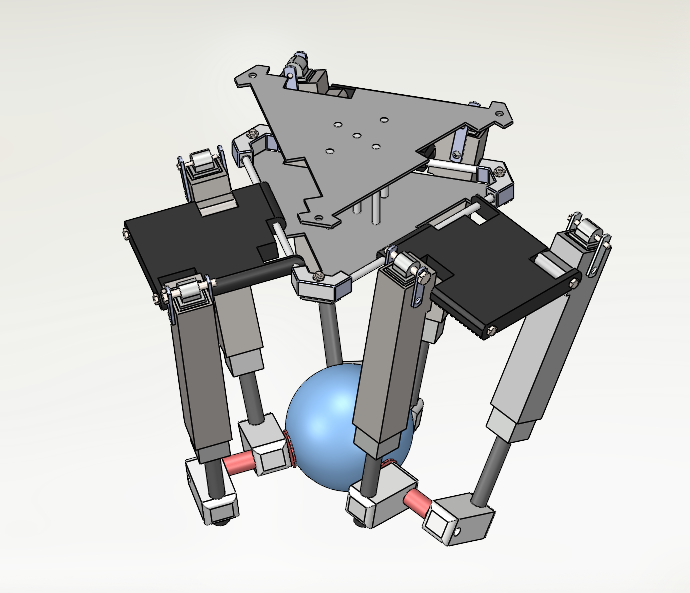
\includegraphics[width=100mm,scale=0.6]{images/Project4/stewart_gripper.png}
    \caption{Novel Parallel robot Griper}
    \label{fig:Parallel}
\end{figure}


\section{Conclusion}
Finally, in Fig. \ref{fig:Parallel}\footnote{Complete model uploaded in \url{https://grabcad.com/library/stewart-manipulator-1}.}  we can observe the final solution proposed with a parallel robot hand, which presents rotation and translation, the prismatic actuators presented and the union of the extremities by means of magnets, generates a better grip on high-density objects, the system is simplified and without redundancies, which implies a greater space for handling and rotation for handling.\\
Compared with conventional robotic hands, this system based on parallel robots presents a greater structural robustness due to the dynamics of the system, in the same way the magnets that are proposed in the ends of the fingers as an initial idea will become a great innovation because they do not Similar ideas are observed even in the market in robotic hands.










\end{document}